%% FLIP-IT — Technical Expert Report
%% Build: pdfLaTeX + bibtex (backend=bibtex, so no biber install needed).  Overleaf: upload this
%% directory, compiler pdfLaTeX; the bibtex step is detected automatically.
%% Every number in the prose comes from generated/macros.tex — never type one in by hand.
%% Regenerate figures, tables and macros with:  uv run python paper/make_paper.py
\documentclass[11pt,a4paper]{article}

\usepackage[T1]{fontenc}
\usepackage[utf8]{inputenc}
\usepackage{lmodern}
\usepackage[english]{babel}
\usepackage[a4paper,margin=2.5cm]{geometry}
\usepackage{microtype}
\usepackage{booktabs}
\usepackage{longtable}
\usepackage{array}
\usepackage{graphicx}
\usepackage{xcolor}
\usepackage{enumitem}
\usepackage{caption}
\usepackage[most]{tcolorbox}
\usepackage{amsmath}
\usepackage{hyperref}

\usepackage[backend=bibtex,style=numeric,sorting=none]{biblatex}
\addbibresource{refs.bib}

\graphicspath{{figures/}}

%% ── palette ────────────────────────────────────────────────────────────────
\definecolor{ink}{HTML}{141D24}
\definecolor{muted}{HTML}{5C6B77}
\definecolor{rule}{HTML}{E3E9ED}
\definecolor{accent}{HTML}{2A78D6}
\definecolor{warn}{HTML}{EB6834}
\definecolor{boxbg}{HTML}{F5F8FB}

\hypersetup{colorlinks=true, linkcolor=accent, urlcolor=accent, citecolor=accent,
  pdftitle={FLIP-IT: Technical Expert Report}, pdfauthor={FLIP-IT technical work package}}

\captionsetup{font=small, labelfont=bf, labelsep=period}
\setlist[itemize]{leftmargin=1.2em, itemsep=2pt, topsep=3pt}
\setlist[enumerate]{leftmargin=1.4em, itemsep=2pt, topsep=3pt}

%% ── the document's three structural devices ────────────────────────────────
%% \question — the section heading IS the question counsel asked.
\newcommand{\question}[1]{\section{#1}}

%% \shortanswer — a boxed one-paragraph answer directly under the heading, so the
%% whole report can be read as a sequence of boxes and stopped there.
\newtcolorbox{answerbox}[1][]{
  enhanced, breakable, colback=boxbg, colframe=accent,
  boxrule=0pt, leftrule=2.5pt, arc=1pt, left=8pt, right=8pt, top=6pt, bottom=6pt,
  fonttitle=\bfseries\small, #1}
\newenvironment{shortanswer}{\begin{answerbox}\small\textbf{Answer.\ }}{\end{answerbox}}

%% \status — every section declares what kind of claim it is making.
\newcommand{\statuschip}[2]{{\small\textcolor{#1}{\textbf{#2}}}}
\newcommand{\statusMethod}{\statuschip{accent}{Methodology-determined}%
  {\small\textcolor{muted}{ true of the method regardless of the data}}\par\medskip}
\newcommand{\statusMeasured}{\statuschip{accent}{Measured on the test bed}%
  {\small\textcolor{muted}{ synthetic data, \NumSeeds{} seeds; see \S\ref{sec:limits}}}\par\medskip}
\newcommand{\statusDeployment}{\statuschip{warn}{Requires the deployment}%
  {\small\textcolor{muted}{ depends on decisions not yet taken}}\par\medskip}
\newcommand{\statusOutside}{\statuschip{warn}{Outside technical scope}%
  {\small\textcolor{muted}{ stated as a boundary, with the facts needed to decide it}}\par\medskip}

%% A marked box for material addressed to another work package rather than to counsel.
\newtcolorbox{sidenote}[1]{enhanced, breakable, colback=white, colframe=muted,
  boxrule=0.6pt, sharp corners, left=8pt, right=8pt, top=6pt, bottom=6pt,
  borderline={0.6pt}{0pt}{muted, dash pattern={on 3pt off 2pt}},
  title={\small\bfseries #1}, coltitle=ink, colbacktitle=white, fonttitle=\bfseries}

% GENERATED by paper/make_paper.py -- do not edit.
% Every number quoted in the report's prose resolves through one of these.
\newcommand{\NumPractices}{10}
\newcommand{\NumPatients}{3,276}
\newcommand{\PanelMin}{161}
\newcommand{\PanelMax}{532}
\newcommand{\PrevMin}{8.3\%}
\newcommand{\PrevMax}{46.0\%}
\newcommand{\NumSeeds}{5}
\newcommand{\HeadlineRound}{20}
\newcommand{\MaxRounds}{50}
\newcommand{\DPRounds}{20}
\newcommand{\CeilingAUC}{0.861}
\newcommand{\BestFedAUC}{0.808}
\newcommand{\BestFedWorst}{0.675}
\newcommand{\LocalAUC}{0.789}
\newcommand{\LocalWorst}{0.495}
\newcommand{\WorstGain}{+0.180}
\newcommand{\CeilingGapAbs}{0.054}
\newcommand{\FedAvgAUC}{0.808}
\newcommand{\MosaicAUC}{0.800}
\newcommand{\UplinkLogreg}{352}
\newcommand{\UplinkMosaic}{3,600}
\newcommand{\NegControlMax}{0.524}
\newcommand{\NegControlCeiling}{0.513}
\newcommand{\EpsAtSigmaTwo}{12.3}
\newcommand{\EpsAtSigmaTwoNaive}{48}
\newcommand{\AUCAtSigmaTwo}{0.773}
\newcommand{\WorstAtSigmaTwo}{0.608}
\newcommand{\EpsAtSigmaOne}{30.1}
\newcommand{\AUCAtSigmaOne}{0.794}
\newcommand{\WorstAtSigmaOne}{0.646}
\newcommand{\LocalEpsFive}{31.4}
\newcommand{\LocalAUCFive}{0.754}
\newcommand{\LocalWorstFive}{0.574}
\newcommand{\LocalEpsOne}{4.3}
\newcommand{\LocalAUCOne}{0.627}
\newcommand{\LocalWorstOne}{0.397}
\newcommand{\LocalVsCentralAUCGap}{0.040}
\newcommand{\LocalVsCentralWorstGap}{0.072}
\newcommand{\NegControlMaxCorr}{0.031}
\newcommand{\MIANoDPThreshold}{0.501}
\newcommand{\MIANoDPShadow}{0.502}
\newcommand{\MIAControlThreshold}{0.655}
\newcommand{\MIAControlShadow}{0.659}
\newcommand{\MIAControlN}{40}
\newcommand{\MIAMargin}{0.02}
\newcommand{\FlwrVersion}{1.33.0}
\newcommand{\RunDate}{2026-08-20}
\newcommand{\NumFeatures}{10}


%% ───────────────────────────────────────────────────────────────────────────
\begin{document}

\begin{titlepage}
\vspace*{2cm}
{\Huge\bfseries FLIP-IT\par}
\vspace{6pt}
{\LARGE Technical Expert Report\par}
\vspace{18pt}
{\large Federated learning for chronic kidney disease risk\\
across regional GP practices\par}
\vspace{24pt}
\noindent\rule{\textwidth}{0.6pt}
\vspace{12pt}

{\large\bfseries In response to:} the preliminary legal assessment of 10 August 2026\\
(J.~Fl\"ototto, Jorzig \& Partner), and the central open technical question\\
transmitted by Dr.~N.~Conze, docport GmbH.

\vspace{18pt}
{\large\bfseries Prepared by:} Dr.~Andy Man Yeung Tai

\vspace{18pt}
{\large\bfseries Status:} Preliminary engineering findings. \textbf{Not legal advice.}\\
This document supplies facts for the legal assessment; it does not draw legal conclusions.

\vspace{12pt}
{\large\bfseries Basis:} \texttt{FL-CKD-Flower}, the pre-kickoff methodology test bed.\\
Verified against Flower \FlwrVersion{}. Measurements are \textbf{synthetic}.\\
Run of \RunDate{} see Appendix~\ref{sec:repro}.

\vspace{12pt}
\noindent\rule{\textwidth}{0.6pt}

\vfill
\begin{answerbox}
\small
\textbf{How to read this report.} Every section heading is a question counsel raised. Directly
under each heading is a boxed one-paragraph answer; the discussion that follows is the reasoning and
the evidence. Reading only the boxes gives a complete, if compressed, set of answers.

Each section also carries a status chip stating what kind of claim it makes:
\textcolor{accent}{\textbf{Methodology-determined}} facts hold regardless of which data the system
runs on; \textcolor{accent}{\textbf{Measured on the test bed}} results come from synthetic data and
transfer only as evidence about the method; \textcolor{warn}{\textbf{Requires the deployment}} marks
questions that no amount of engineering here can close.
\end{answerbox}
\end{titlepage}

%% Scope remark (2026-08-28): the test-bed codebase was reduced to logistic regression only after
%% the pinned run of \RunDate{}; the MLP and XGBoost/FedXgbBagging paths were evaluated and deleted.
%% Table rows, figure series and prose naming the removed protocols are historical measurements,
%% pending regeneration via make_paper.py --recompute over the logreg-only code. This file is
%% hand-authored (make_paper.py generates figures/, tables/ and generated/ only), so the note
%% lives here rather than in the pipeline.
\noindent\textbf{Scope note (2026-08-28).} The \texttt{FL-CKD-Flower} codebase was reduced to
logistic regression only after the pinned run of \RunDate{} behind this report: the MLP and the
tree-based federated protocol were evaluated and then deleted from the code. Table rows, figure
series and passages naming those removed protocols are historical measurements, pending
regeneration over the logistic-regression-only repository.

\tableofcontents
\newpage

\section*{Scope, and what changed since the assessment}
\addcontentsline{toc}{section}{Scope, and what changed since the assessment}

The preliminary legal assessment of 10 August 2026 put one central technical question to this work
package, and listed four items under GDPR Art.~4(1) \cite{gdpr} as \emph{not yet conclusively
documented}: the privacy budget and DP configuration; the number and size of participating cohorts;
the training and aggregation configuration; and the administrative access, logging and export
capabilities on the SuperLink. It further noted that the effectiveness of the protective mechanisms
had not been demonstrated by any documented anonymisation or re-identification test.

Rather than document those gaps, we closed the ones within our control and then wrote this report
against the resulting system. Since the assessment:

\begin{itemize}
  \item \textbf{Secure aggregation is implemented} and verified end-to-end, so the answer to the
        central question is now a configuration choice rather than a limitation (\S\ref{sec:secagg}).
  \item \textbf{Noise at the practice is implemented and measured} --- the only mechanism that
        changes what the aggregating party receives (\S\ref{sec:noise}).
  \item \textbf{The privacy budget is now computed by a standard accountant} rather than by a
        hand-rolled bound that was, at low noise, not a valid bound at all (\S\ref{sec:budget}).
  \item \textbf{A membership-inference audit exists} and reports attack results against the released
        model (\S\ref{sec:anontest}).
  \item \textbf{The direct identifier is gone} from the practice export, and per-practice metric
        logging is anonymised by default (\S\ref{sec:sidechannels}).
\end{itemize}

\paragraph{What this report is.} \texttt{FL-CKD-Flower} is the \textbf{methodology test bed} for
FLIP-IT. No live deployment exists, no real patient data has ever entered it, and every measurement
below comes from \NumPractices{} synthetic practices totalling \NumPatients{} generated patients.
The \emph{method} is therefore described definitively --- that is what counsel needs in order to
assess it --- while \emph{measurements} are labelled as test-bed evidence. The status chip on each
section keeps the two apart, and \S\ref{sec:realdata} states explicitly which conclusions survive the
move to real practice data and which do not.

\paragraph{What this report is not.} It is not legal advice, and it does not conclude whether a
gradient is personal data. That is counsel's determination; this document supplies the technical
facts it rests on.

\subsection*{Answers at a glance}

\begin{longtable}{p{0.36\textwidth}p{0.44\textwidth}p{0.12\textwidth}}
\toprule
\textbf{Question} & \textbf{Answer} & \textbf{Status} \\
\midrule
\endhead
Does the SuperLink ever hold one practice's update in isolation? (\S\ref{sec:isolation})
  & On the default configuration, yes --- in the clear and attributable. Under secure aggregation,
    no. It is a configuration state, not an architectural limit.
  & Method \\
\addlinespace
Does Flower Labs receive anything? (\S\ref{sec:flowerlabs})
  & No. The SuperLink is self-hosted; the company has no access path. One CLI default has been
    removed as a precaution.
  & Method \\
\addlinespace
Is secure aggregation reachable? (\S\ref{sec:secagg})
  & Yes, and it is now built and verified. Semi-honest threat model; participation stays visible.
  & Method \\
\addlinespace
Where can noise be added, and what does each placement protect? (\S\ref{sec:noise})
  & Central DP constrains the published model but leaves the server seeing un-noised updates. Only
    local DP changes that --- and it is expensive.
  & Measured \\
\addlinespace
What is the privacy budget? (\S\ref{sec:budget})
  & $\varepsilon = \EpsAtSigmaTwo$ at $\sigma = 2.0$ over \DPRounds{} rounds, by an RDP accountant.
    The previously circulated figures were invalid, not merely loose.
  & Measured \\
\addlinespace
How is $\varepsilon$ reduced without losing accuracy? (\S\ref{sec:reduce})
  & Fewer rounds --- convergence is reached by round~10, so halving the round count halves the
    budget for nothing. Then more practices.
  & Measured \\
\addlinespace
Can aggregated results be de-aggregated? (\S\ref{sec:aggdisclosure})
  & For the training path, addressed. For the analytics path the structural answers carry over, but
    the disclosure-control questions need that component's indicator specification.
  & Method \\
\addlinespace
Does the system disclose anything outside the model path? (\S\ref{sec:sidechannels})
  & It did, in two places. Both are now closed by default.
  & Method \\
\addlinespace
Does federation actually work? (\S\ref{sec:works})
  & Within \CeilingGapAbs{} AUROC of the pooled ceiling, and it lifts the worst practice by
    \WorstGain{}. The benefit is equity, not average accuracy.
  & Measured \\
\addlinespace
Has anonymisation been demonstrated by test? (\S\ref{sec:anontest})
  & Partly. Membership inference finds no usable signal --- even with no DP --- and the positive
    control confirms the attack works. Two of the three attack families EDPB names remain unbuilt.
  & Measured \\
\addlinespace
What is actually configured on the SuperLink? (\S\ref{sec:outside})
  & Unanswerable here. We document the full capability surface; the operator's choices are not ours
    to state.
  & Deployment \\
\bottomrule
\end{longtable}

\subsection*{Where each concern is answered}

\begin{longtable}{p{0.50\textwidth}p{0.42\textwidth}}
\toprule
\textbf{Raised in the assessment} & \textbf{Answered in} \\
\midrule
\endhead
Central open technical question --- isolated access to individual contributions
  & \S\ref{sec:isolation}, \S\ref{sec:secagg}, \S\ref{sec:flowerlabs} \\
Art.~4(1) item 1 --- privacy budget $\varepsilon$/$\delta$ and DP configuration
  & \S\ref{sec:noise}, \S\ref{sec:budget}, \S\ref{sec:reduce}, App.~\ref{sec:config} \\
Art.~4(1) item 2 --- number and size of participating cohorts
  & \S\ref{sec:works}, App.~\ref{sec:config} \\
Art.~4(1) item 3 --- training and aggregation configuration
  & \S\ref{sec:method}, App.~\ref{sec:config} \\
Art.~4(1) item 4 --- administrative access, logging, export on the SuperLink
  & \S\ref{sec:outside} (capability surface documented; operator configuration out of scope) \\
No documented anonymisation or re-identification test
  & \S\ref{sec:anontest} \\
Gradients may retain training-set information
  & \S\ref{sec:payload}, \S\ref{sec:anontest} \\
Analytics path --- cell counts, suppression, de-aggregation, repeated analyses
  & \S\ref{sec:aggdisclosure} (structural answers; indicator spec required) \\
Art.~26/28 role allocation, DPIA, AI Act
  & \S\ref{sec:outside} \\
\bottomrule
\end{longtable}

\question{What does FLIP-IT compute, and where does each step happen?}
\label{sec:method}
\statusMethod

\begin{shortanswer}
Every computation that touches a patient row happens inside the practice. Each round, a practice
receives the current global coefficient vector, trains on its own rows for two passes, and returns
an updated vector plus the number of examples it trained on. The server multiplies those vectors by
their example counts, sums, and divides. No patient row, and no derived per-patient quantity, is
ever transmitted --- including the feature scaler, which is fitted locally and stays there.
\end{shortanswer}

\subsection{The local pipeline}

A practice's SuperNode holds its own extract and never sends it anywhere. Per round, in order:

\begin{enumerate}
  \item \textbf{Load} the practice's rows. In the pilot this is the practice's own FHIR server or
        its Tomedo export; in the test bed it is a generated CSV. The loader is the only component
        that differs, deliberately, so that everything downstream is identical either way.
  \item \textbf{Split} 80/20 into train and held-out, by a permutation seeded from the global seed
        and the practice index --- reproducible, and stable across rounds so that the held-out rows
        are never trained on.
  \item \textbf{Scale} features with a \texttt{StandardScaler} fitted \emph{on this practice's
        training rows only}. This matters for the disclosure analysis: the scaler encodes practice
        means and variances, and it is \textbf{never transmitted}. Each practice keeps its own.
  \item \textbf{Train} logistic regression, warm-started from the global vector, for two full
        passes, with balanced class weighting for the prevalence imbalance.
  \item \textbf{Reply} with the updated coefficient vector and \texttt{num-examples}.
\end{enumerate}

The model is logistic regression over \NumFeatures{} features plus an intercept: age, six binary
comorbidity flags, and three ``years since diagnosis'' durations. \S\ref{sec:modelchoice} explains
why this model class rather than a stronger one, and why that choice is also the privacy-preferable
one.

\subsection{The round trip}

FLIP-IT runs on Flower \cite{beutel2020flower}, version \FlwrVersion{}. In the deployment runtime the
\textbf{SuperLink} is a message broker: practices (\textbf{SuperNodes}) pull instruction messages and
push reply messages; the ServerApp retrieves the replies and aggregates them. The aggregation rule
is sample-weighted federated averaging \cite{mcmahan2017fedavg}: with $w_i$ the vector returned by
practice $i$ and $n_i$ its example count,
\[
  w_{\text{global}} \;=\; \frac{\sum_i n_i\, w_i}{\sum_i n_i}.
\]
\texttt{num-examples} is exactly the $n_i$ above --- it is transmitted because the average is
weighted by it, and for no other purpose.

Two properties of this arrangement drive the whole of \S\ref{sec:isolation}, and they are worth
stating here rather than as a surprise later: \textbf{aggregation is the last step of a round, not a
property of transmission}, and \textbf{every message carries its sender's identity}. Neither is a
defect; both are simply how the protocol works, and both are what secure aggregation exists to
change.

\subsection{Configuration}

The complete training and aggregation configuration --- the third of the four items the assessment
listed as undocumented --- is a single declarative block in the project's \texttt{pyproject.toml},
reproduced in full in Appendix~\ref{sec:config}. It is not scattered through code, and it is
versioned with the code it configures, so any run's configuration is recoverable from the commit
that produced it.

\question{What crosses the practice boundary, and what does it contain?}
\label{sec:payload}
\statusMeasured

\begin{shortanswer}
On the recommended configuration, \UplinkLogreg{} bits per practice per round: eleven coefficients
and an intercept. That vector is fitted to this practice's patients and is the object that
gradient-inversion research targets, so treating it as carrying information about those patients is
correct. A second, \emph{historical alternative} was materially worse: the tree-based protocol (FedXgbBagging,
evaluated on this report's pinned run and \textbf{deleted from the codebase on 2026-08-28} --- see
the scope note in the front matter) transmitted serialized trees whose split thresholds were
\emph{literal patient feature values} --- the highest-disclosure payload in the comparison and the
one secure aggregation cannot protect. What remains is the comparison between the two
logistic-regression protocols below.
\end{shortanswer}

\begin{table}[htbp]
  \centering
  \caption{What each protocol places on the wire, per practice per round. Measured in the test bed.}
  \begin{tabular}{lp{7.4cm}r}
    \toprule
    Protocol & What crosses the practice boundary & Bits/round \\
    \midrule
    FedProx & model coefficients --- a parameter vector fitted to this practice's patients & 352 \\
    FedMosaic & predictions + expertise on a \emph{public} cohort --- no parameter vector & 3,600 \\
    FedXgbBagging & serialized decision trees --- split thresholds are literal patient values & 21,521 \\
    \bottomrule
\end{tabular}

  \label{tab:payload}
\end{table}

\begin{figure}[htbp]
  \centering
  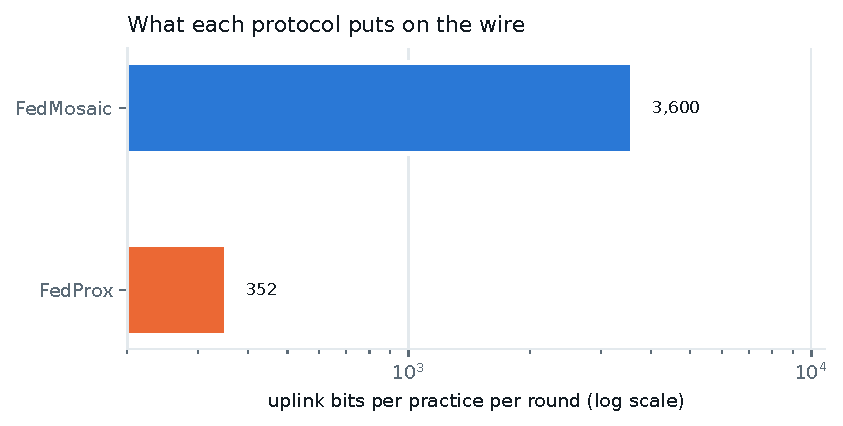
\includegraphics[width=0.82\textwidth]{payload}
  \caption{Uplink volume per practice per round, log scale, for the two logistic-regression
  protocols. (The pinned run also measured a tree-based protocol at roughly sixty times the
  coefficient vector; that series is historical --- the model was removed from the codebase on
  2026-08-28.)}
  \label{fig:payload}
\end{figure}

\subsection{Why the payload's \emph{shape} matters, not just its size}

The three protocols differ in kind, not only in degree:

\begin{itemize}
  \item \textbf{Coefficients} (FedProx, FedAvg) are an aggregate summary: each number is a
        partial derivative averaged over hundreds of patients. Inverting them to recover an
        individual is the subject of the gradient-leakage literature \cite{zhu2019leakage}.
  \item \textbf{Serialized decision trees} (FedXgbBagging -- \emph{historical}: this protocol was
        evaluated and removed from the codebase on 2026-08-28) are categorically different. A split
        threshold such as \emph{age $\le$ 67.5} is derived directly from patient values present in
        that practice's data. There is no averaging step to hide behind.
  \item \textbf{Predictions on a public cohort} (FedMosaic \cite{fedmosaic}) are different again.
        The practice transmits opinions about patients who are \emph{already public}, plus an
        expertise weight. No parameter vector exists for the server to invert.
\end{itemize}

\subsection{How much can a coefficient vector reveal?}

The gradient-inversion results counsel's assessment alludes to were established against deep
networks with millions of parameters, where a single update can carry enough information to
reconstruct an input image. The object here is different by orders of magnitude: \textbf{eleven
parameters}, averaged over a practice's entire training set, in a \emph{convex} optimisation whose
optimum is a property of the dataset as a whole rather than of any record in it.

That is an argument for lower risk, and it should be stated as an argument not as a conclusion.
It is exactly the kind of claim EDPB Opinion 28/2024 \cite{edpb2024ai} declines to accept without
testing, which is why \S\ref{sec:anontest} tests it rather than asserting it. The measured result
there is consistent with this reasoning, and its limits are stated with it.

\question{Does the SuperLink, or Flower Labs, at any point have isolated access to individual
practices' contributions or is only the joint aggregate ever accessible?}
\label{sec:isolation}
\statusMethod

\begin{shortanswer}
This is the central question the assessment put to us, and it has two answers depending on one
configuration switch. \textbf{On the default configuration, the aggregating party receives each
practice's update in the clear, attributable to that practice.} Secure aggregation is not active by
default, so counsel's premise ``as a result of the secure aggregation implementation'' did
not describe the system as it stood. \textbf{With \texttt{secure-aggregation} enabled, it does:} the
server can open only the sum, never one practice's contribution (\S\ref{sec:secagg}). This is
therefore a decision to be taken, not an engineering limitation. Flower Labs, the company, receives
nothing in either case (\S\ref{sec:flowerlabs}).
\end{shortanswer}

\subsection{Why the default answer is what it is}

Two structural facts, both verified against the installed package rather than inferred from
documentation.

\paragraph{(a) Aggregation is the last step, not a property of transmission.}
In Flower's deployment runtime the SuperLink is a message broker. SuperNodes push reply messages to
its Fleet API and the ServerApp retrieves them. The aggregation function receives a \emph{list of
individual messages}, each carrying that practice's own array record the raw parameter vector
and only then combines them. Sending an update to the server does not aggregate it. There is a
moment, by construction, at which the aggregating party holds $n$ separate vectors.

\paragraph{(b) Each message is individually attributable.}
Every Flower message carries \texttt{metadata.\allowbreak src\_\allowbreak node\_\allowbreak id}, and the framework's own aggregation
code reads it. A practice's update is not an anonymous contribution to a pool: it arrives tagged
with the identity of the SuperNode that sent it, which under the authentication scheme in the
deployment guide is bound by public key to a named practice. The node registry that maps keys to
admitted practices is centrally held.

Together: at the moment of aggregation, the aggregating party holds \emph{this named practice's
parameter vector, derived from this named practice's patients.}

\subsection{What this does and does not imply}

Two qualifications, pulling in opposite directions, and both belong here.

\textbf{It is a configuration state.} Federated learning does not
require the server to see individual contributions. The mechanisms that prevent it were switched off
in a research baseline, deliberately, so that reference numbers stayed interpretable. They are now
implemented and can be switched on.

\textbf{But nothing in the default configuration supports a claim of anonymity at the aggregation
level.} The conservative treatment the assessment recommends treating gradients as personal
data, and potentially as health data is the technically correct treatment of the system running
in its default configuration, and we do not argue against it on that configuration. What
\S\ref{sec:secagg} and \S\ref{sec:noise} change is the set of configurations available to choose from.

\subsection{A note on the two data paths}

The assessment distinguishes a \emph{federated analytics} path carrying aggregated indicator vectors
from an \emph{AI training} path carrying gradients, and assigns them different legal prospects. It
is worth recording that \textbf{this distinction is not an architectural boundary in Flower}: the
term ``analytics'' does not occur anywhere in the installed package, which offers one message API
and one strategy interface. Both paths would be the same mechanism a client returning a record
to a server through the SuperLink and therefore the two structural facts above apply to the
analytics path unchanged.

\question{Does Flower Labs, the company, receive anything?}
\label{sec:flowerlabs}
\statusMethod

\begin{shortanswer}
No. In the intended deployment the SuperLink is self-hosted on consortium infrastructure and Flower
is open-source software running on that host; the company has no access path and receives nothing.
One caveat was worth closing rather than explaining: the Flower CLI writes a default entry pointing
at a Flower-operated endpoint into a freshly generated configuration file. It is inert unless
explicitly invoked, but it is one word on a command line, so its removal is now a documented step on
the practice-side go-live checklist.
\end{shortanswer}

\subsection{The configuration default, and why it was closed}

A newly generated \texttt{\$HOME/.flwr/config.toml} contains, among the connection profiles:

\begin{quote}\ttfamily
[superlink.supergrid]\\
address = "supergrid.flower.ai"
\end{quote}

Nothing routes there unless someone runs the deployment command naming that profile explicitly. But
the gap between a self-hosted federation and transmission of model updates to a third party should
not be a single word on a command line that a tired operator could type. The deployment procedure now
requires removing the entry on every operator and practice machine and pinning the default profile to
the consortium SuperLink, so that an omitted argument also cannot reach outside the consortium. It is
cheap to do and easy to forget, which is why it is on a checklist rather than in prose.

\subsection{The Letter of Intent}

The Projektantrag \cite{projektantrag} records a Letter of Intent from FlowerAI. It concerns
technical support and expertise. \textbf{It is not a data-processing arrangement and should not be
relied on as one.} If any future configuration were to route data through infrastructure Flower Labs
operates, that would be a new processing relationship requiring its own legal basis, and it is not
what is planned.

\question{Is secure aggregation reachable, and what exactly does it guarantee?}
\label{sec:secagg}
\statusMethod

\begin{shortanswer}
It is reachable, and it is now implemented and verified end-to-end: with
\texttt{secure-aggregation} enabled, a full round of training and evaluation completes across twelve
practices and the server obtains only the sum. Three limits must travel with any claim made about
it. The guarantee is \textbf{semi-honest} --- it protects against a server that follows the protocol
and inspects what it receives, not against one that deviates. \textbf{Participation stays visible}:
the server always learns who took part. And \textbf{the aggregate is still model parameters}, so
secure aggregation does not by itself make the released model anonymous.
\end{shortanswer}

\subsection{The mechanism}

Secure aggregation \cite{bonawitz2017secagg} has each pair of participating practices derive a
shared secret mask. Practice $i$ adds the mask to its update and practice $j$ subtracts it, so the
masks cancel exactly when the contributions are summed --- and only then. The server sees each
practice's masked vector, which on its own is indistinguishable from noise, and recovers a
meaningful value only from the total.

Because a practice that drops out mid-round would leave its masks uncancelled, each practice also
distributes Shamir secret shares of its own seed. If enough surviving practices contribute shares,
the dropped practice's mask can be reconstructed and removed. Two parameters govern this and are
exposed as configuration: the number of shares issued per practice, and the reconstruction threshold
--- the number required to recover a mask. The threshold is the security parameter: it is the number
of practices that would have to collude \emph{with} the server to unmask an individual contribution.

\subsection{Why it is a second code path}

\begin{table}[htbp]
  \centering
  \caption{Secure-aggregation availability, probed against the installed package rather than
  assumed from documentation.}
  \begin{tabular}{lp{5.2cm}}
    \toprule
    Probe & Result \\
    \midrule
    \texttt{secaggplus\_mod} in \texttt{flwr.clientapp.mod} (Message API) & absent \\
    \texttt{secaggplus\_mod} in \texttt{flwr.client.mod} (legacy) & present \\
    \texttt{SecAggPlusWorkflow} importable & present \\
    \texttt{SecAggPlusWorkflow} requires \texttt{LegacyContext} & yes \\
    DP mods in \texttt{flwr.clientapp.mod} & \texttt{fixedclipping\_mod}, \texttt{adaptiveclipping\_mod}, \texttt{LocalDpMod} \\
    Implemented and verified in this repository & yes \\
    \bottomrule
\end{tabular}

  \label{tab:secagg}
\end{table}

In Flower \FlwrVersion{}, secure aggregation ships only in the \emph{legacy} namespaces: the client
modifier is absent from the current message-API namespace, and the workflow that drives it demands a
legacy context. It therefore cannot compose with the strategy entry point this project's server
otherwise uses. It \emph{is} reachable by driving the legacy workflow from inside the modern server
application, and that is what is now built.

Two implementation notes, recorded because they are the kind of detail that is expensive to
rediscover:

\begin{itemize}
  \item \textbf{One client application serves both paths.} The legacy workflow speaks a different
        record shape than the message API, so the practice's handlers accept either and translate
        through Flower's own compatibility bridge. There is no duplicated training code.
  \item \textbf{The switch is ordinary run configuration, not an environment variable.} Client
        modifiers are attached at construction time, before any run configuration exists, so secure
        aggregation and local DP are each installed as a small dispatching modifier that reads the
        configuration when it is called. This also makes them survive the process boundary in
        simulation, where client applications run in worker processes that do not inherit the
        launching environment.
\end{itemize}

\subsection{The three limits, stated plainly}

\begin{enumerate}
  \item \textbf{The threat model is semi-honest.} The guarantee holds against a server that follows
        the protocol but inspects what it receives. It is \emph{not} a guarantee against a server
        that actively deviates --- most obviously by running a round with a single practice, whose
        ``aggregate'' is that practice's update. The available control is the minimum participant
        count, which is set to the full practice count so that such a round fails rather than
        quietly succeeding. That is a configuration discipline, not a cryptographic guarantee, and
        counsel should treat it as such.
  \item \textbf{Participation stays visible.} The server always learns which practices took part in
        each round, and the aggregate. Only the individual contribution is hidden. Where
        participation itself is sensitive --- a practice's presence in a CKD study may be --- secure
        aggregation does not address it.
  \item \textbf{The aggregate is still model parameters.} Secure aggregation answers \emph{who may
        see one practice's update}. It says nothing about what can be inferred from the model that
        is eventually released. That is the province of \S\ref{sec:budget} and \S\ref{sec:anontest}.
\end{enumerate}

\subsection{One protocol it cannot protect}

Secure aggregation masks numeric vectors by arithmetic that cancels on summation. The tree-based
protocol transmits serialized decision trees, which are not a numeric vector and cannot be summed;
there is nothing to mask. \textbf{Any secure-aggregation deployment is necessarily a
logistic-regression deployment.} As \S\ref{sec:modelchoice} shows, the accuracy evidence points the
same way independently, so this constraint costs nothing.

\question{Where can noise be added, and what does each placement actually protect?}
\label{sec:noise}
\statusMeasured

\begin{shortanswer}
This is the single most important technical distinction in this report. \textbf{Central DP does not
answer the central question.} Its noise is applied by the server \emph{as it aggregates}, so the
server necessarily receives every practice's un-noised update first; it constrains what can be
inferred from the published model, not what the aggregating party sees. What changes that is noise
added \textbf{inside the practice's own SuperNode, before transmission}. The update-level local DP
we first measured is unusable at a defensible budget (worst practice \LocalWorstOne{} at composed
$\varepsilon \approx \LocalEpsOne{}$, below the \LocalWorst{} it scores by not collaborating at
all). The deployment standard now delivers the workable form: \textbf{record-level DP-SGD inside
each practice}, with a rule-based server planner setting each practice's batch size and noise
multiplier so every practice composes to one shared target $\varepsilon^{*}$. The measured utility
is flat from $\varepsilon^{*} = 0.5$ to $8$ (Table~\ref{tab:dpsgdstandard}); it composes with
secure aggregation (\S\ref{sec:secagg}).
\end{shortanswer}

\subsection{Three placements, two of which change what the server receives}

\begin{table}[htbp]
  \centering
  \small
  \begin{tabular}{lp{4.0cm}p{3.4cm}l}
    \toprule
    Mechanism & Where the noise is applied & Server still sees the individual update? & Status \\
    \midrule
    Central DP & Server, \emph{during} aggregation & \textbf{Yes un-noised} & measured \\
    Local DP (update-level) & Inside the SuperNode, before transmission & No noised at source & measured \\
    \textbf{Record-level DP-SGD (standard)} & \textbf{Inside the SuperNode, per patient record, before transmission} & \textbf{No per-record gradients clipped and noised at source} & \textbf{measured} \\
    Secure aggregation & Cryptographic masking across practices & No only the sum & implemented \\
    \bottomrule
  \end{tabular}
  \caption{Only the in-practice rows change what the aggregating party receives. This distinction is
  easy to lose and it is the crux of the assessment's central question.}
  \label{tab:placements}
\end{table}

\subsection{A naming trap that inverts the answer}

Flower also ships a strategy named \texttt{DifferentialPrivacyClientSideFixedClipping}. Its own
documentation describes it as \emph{``central DP with client-side fixed clipping''}: only the
\textbf{clipping} moves to the client, while the \textbf{noise is still added by the server}. A
reviewer scanning the API for ``client-side DP'' would conclude the server no longer sees un-noised
updates, and would be wrong. We flag it explicitly because the mistake is natural and the
consequence is a false statement to a regulator.

The mechanism that does what its name suggests is the local DP modifier, which clips the update and
adds Gaussian noise with standard deviation
$\sigma = \text{sensitivity} \cdot \sqrt{2\ln(1.25/\delta)}\,/\,\varepsilon$
inside the SuperNode. It is parameterised by $(\varepsilon, \delta)$ directly rather than by a raw
noise scale.

\subsection{What update-level local DP costs, measured}

\begin{table}[htbp]
  \centering
  \caption{Update-level local DP: noise added inside the SuperNode. $\varepsilon$ is the modifier's own per-round
  parameter; the composed column is the budget over \DPRounds{} rounds from the same accountant used
  in \S\ref{sec:budget}. \NumSeeds{} seeds, mean $\pm$ s.d.}
  \begin{tabular}{rrrrr}
    \toprule
    $\varepsilon$ per round & $\varepsilon$ composed & AUROC & Worst practice & AUROC cost \\
    \midrule
    off & --- & 0.808 $\pm$ 0.008 & 0.675 $\pm$ 0.054 & --- \\
    50 & 1283.4 & 0.806 $\pm$ 0.008 & 0.677 $\pm$ 0.044 & -0.002 \\
    20 & 257.6 & 0.791 $\pm$ 0.017 & 0.650 $\pm$ 0.052 & -0.017 \\
    10 & 85.0 & 0.768 $\pm$ 0.041 & 0.597 $\pm$ 0.061 & -0.040 \\
    5 & 31.4 & 0.754 $\pm$ 0.009 & 0.574 $\pm$ 0.053 & -0.054 \\
    1 & 4.3 & 0.627 $\pm$ 0.057 & 0.397 $\pm$ 0.130 & -0.181 \\
    \bottomrule
\end{tabular}

  \label{tab:dplocal}
\end{table}

\begin{figure}[htbp]
  \centering
  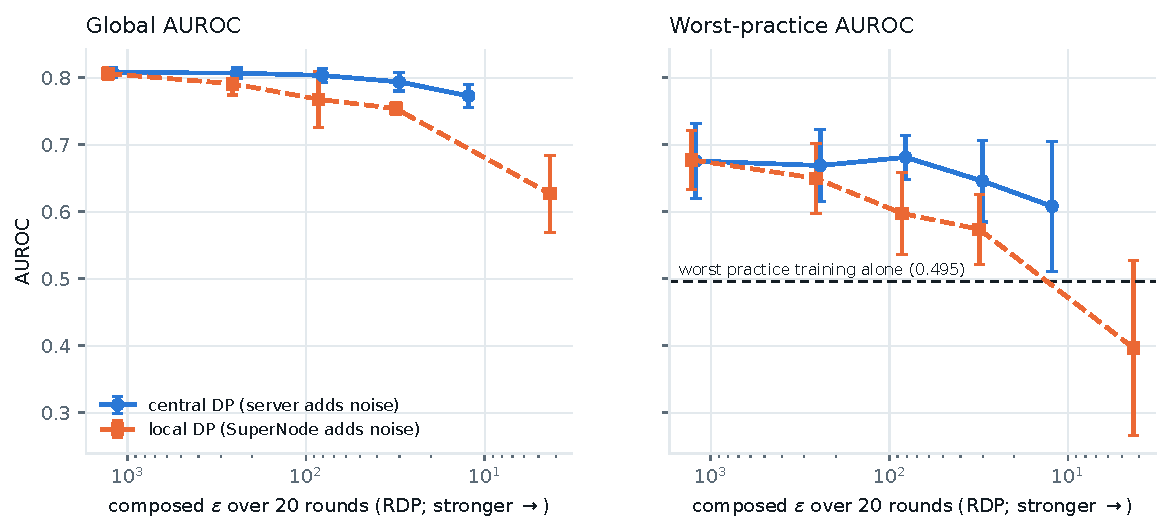
\includegraphics[width=\textwidth]{dp_tradeoff}
  \caption{Utility against budget, both mechanisms on one scale. Stronger privacy is to the right.
  The gap between the curves is the price of the server never holding an individual update if the
  protected unit stays the practice's whole update. Record-level DP-SGD
  (Table~\ref{tab:dpsgdstandard}) closes most of that gap by moving the protected unit to the patient
  record; it is not drawn here because its noise enters during training, not on a released update.}
  \label{fig:dp}
\end{figure}

The comparison that matters is at matched budget. At a composed $\varepsilon$ near
\EpsAtSigmaOne{}, central DP holds global AUROC at \AUCAtSigmaOne{} with worst practice
\WorstAtSigmaOne{}; local DP at a comparable \LocalEpsFive{} reaches only \LocalAUCFive{} and
\LocalWorstFive{}. Roughly \textbf{\LocalVsCentralAUCGap{} AUROC and \LocalVsCentralWorstGap{} worst-practice}
is the measured price.

The reason is structural, not incidental. Under local DP each of the \NumPractices{} practices adds
\emph{independent} noise, so the noise entering the aggregate grows with the number of practices
rather than being added once. Averaging reduces it, but only as $1/\sqrt{n}$ against a noise budget
that each practice must satisfy alone.

\subsection{The resolution: record-level DP-SGD inside the practice}

The update-level finding stands and is worth stating plainly: at $\varepsilon \approx \LocalEpsOne{}$
update-level local DP takes global AUROC to \LocalAUCOne{} and the worst practice to
\LocalWorstOne{}, while a practice that trains entirely alone reaches \LocalWorst{}. \textbf{At
this cohort size, update-level local DP at a meaningful budget produces a model worse than not
collaborating.} The failure is of that mechanism, not of noise-at-the-practice itself, and the
deployment standard now shows the difference: move the protected unit from the practice's
\emph{update} to the patient \emph{record}.

The standard is record-level DP-SGD \cite{abadi2016dpsgd} trained inside each practice's SuperNode.
Every record contributes its own (unweighted)
logistic gradient $(p_i - y_i)\,[x_i, 1]$, clipped to norm $C = 1.0$; Gaussian
noise scaled by $\sigma C$ is added once to the clipped lot sum; optimisation proceeds on
Poisson-sampled lots of size $b$ drawn from the practice's census $N$ (sampling rate $q = b/N$).
The accounted event chain is therefore the sampled Gaussian mechanism, composed with the same
R\'enyi-DP accountant as \S\ref{sec:budget} \cite{mironov2017rdp,dpaccounting} so small and
large practices spend budget in identical units.
% deliberate change (2026-08-27 audit): the privacy-charged mechanism does NOT fold balanced
% class weights into the per-record gradient -- they are computed from local label counts, so
% one added/removed record would change every record's weight and push add/remove-one-record
% sensitivity past one clipped term. Class-balanced weighting stays on the non-DP paths.

One consequence is invisible until measured: a \emph{uniform} $(b, \sigma)$ configuration does not
deliver a uniform budget. At batch~64, $\sigma = 1.5$, ten local epochs and ten rounds the composed
$\varepsilon$ is 1.10 for a 50,000-patient practice but 16.04 for a 500-patient one
(\texttt{orchestrator.uniform\_settings\_audit}); under this report's deployment schedule (two local epochs, ten
rounds) the same flat instruction delivers $\varepsilon = 7.25$ at the cohort's largest practice
and 15.26 at its smallest (the 1.10/16.04 pair is a toy schedule at ten local epochs with
50,000- and 500-patient endpoints, kept to expose the mechanism's size dependence). The large practices are over-protected and the small ones under-protected, and nobody
knows which budget they personally trained under. The standard therefore pairs DP-SGD with a
\textbf{rule-based server-side planner} (a rule table, not a model; no LLM anywhere): R1~reads each
practice's census $N$, the only datum exchanged; R2~fixes one global $(\varepsilon^{*},\,
\delta = 10^{-5})$ policy for the run; R3~inverts the shared accountant per practice for the batch
size and the smallest $\sigma$ whose composed budget stays at or below $\varepsilon^{*}$; R4~dispatches
each practice's plan ($b$, $\sigma$, $C$, local epochs) as run configuration. Every planned practice
is re-verified against the target before dispatch at $\varepsilon^{*} = 2$ the planned $\sigma$
spans 8.32--11.68 across the ten practices, smallest census carrying the largest noise, and every
practice certifies $\varepsilon \le 2.0$.

\begin{table}[htbp]
  \centering
  \caption{The deployment standard, measured: record-level DP-SGD inside each practice with
  per-practice $(b, \sigma)$ orchestrated to one target $\varepsilon^{*}$. \NumPractices{} synthetic
  practices, \NumSeeds{} seeds, $R = 10$ rounds, 2 local epochs, $\delta = 10^{-5}$; mean $\pm$ s.d.
  Computed in \texttt{notebooks/03\_dpsgd\_secagg\_standard.ipynb} \S5, quoted verbatim (not from
  this report's macro cache). The no-DP row re-runs the same DP-SGD runner with $\sigma = 0$; the
  published no-DP FedAvg figure (\BestFedAUC{} / \BestFedWorst{}, \S\ref{sec:works}) used the
  full-batch 20-round path and sits about 0.01 higher a per-sample-clipping path difference, present
  at every budget including none, documented in the notebook.}
  % HAND-AUTHORED -- the deployment-standard sweep lives in notebooks/03_dpsgd_secagg_standard.ipynb,
% outside the make_paper.py cache. Numbers below are that notebook's §5 sweep, quoted verbatim.
\begin{tabular}{lcc}
  \toprule
  Target $\varepsilon^{*}$ & Global AUROC & Worst-practice AUROC \\
  \midrule
  no DP ($\sigma = 0$)      & $0.796 \pm 0.010$ & $0.659 \pm 0.050$ \\
  $\varepsilon^{*} = 0.5$   & $0.798 \pm 0.008$ & $0.660 \pm 0.051$ \\
  $\varepsilon^{*} = 2$     & $0.797 \pm 0.011$ & $0.649 \pm 0.060$ \\
  $\varepsilon^{*} = 8$     & $0.798 \pm 0.011$ & $0.656 \pm 0.050$ \\
  \bottomrule
\end{tabular}

  \label{tab:dpsgdstandard}
\end{table}

Utility is flat: $\varepsilon^{*} = 0.5$ already matches the same-runner no-DP row on both columns,
and $\varepsilon^{*} = 8$ is statistically indistinguishable from it. Against the anchors, that
row (0.797 / 0.649 at $\varepsilon^{*} = 2$) beats central DP at comparable-defensibility settings
(\AUCAtSigmaTwo{} / \WorstAtSigmaTwo{} at composed $\varepsilon \approx \EpsAtSigmaTwo$,
\S\ref{sec:budget}) while also
answering the question central DP cannot, and it replaces update-level local DP's
\LocalAUCOne{} / \LocalWorstOne{} at
$\varepsilon \approx \LocalEpsOne{}$ a setting below the do-nothing floor of training alone. The
small-cohort problem this section opened with is not abolished (the planned $\sigma$ above shows the
smallest practices still paying for their size), but it is relocated from ``is privacy reachable at
all'' to ``which $\varepsilon^{*}$ is the policy choice''; \S\ref{sec:reduce} takes that up, and the
combination with secure aggregation (\S\ref{sec:secagg}) has been verified live.

\begin{sidenote}{Not yet implemented}
FedMosaic specifies its own per-round DP construction an XOR mechanism on the label matrix and
Gaussian noise on the expertise vector. This test bed does not implement it, so FedMosaic's privacy
case here rests on payload shape alone (\S\ref{sec:payload}), not on a formal guarantee.
\end{sidenote}

\question{What is the privacy budget, how is it accounted, and what does it cost?}
\label{sec:budget}
\statusMeasured

\begin{shortanswer}
At clipping norm 1.0 and $\delta = 10^{-5}$ over \DPRounds{} rounds, the budget ranges from
effectively unbounded down to $\varepsilon = \EpsAtSigmaTwo{}$ at noise multiplier $\sigma = 2.0$,
where global AUROC is \AUCAtSigmaTwo{}. These figures come from a R\'enyi-DP accountant. They
supersede the figures circulated previously, which were computed by a hand-rolled composition that
was not merely loose but --- at low noise --- \textbf{outside the range in which the underlying
formula is valid at all}. The mechanism has not changed; only the accounting is now correct.
\end{shortanswer}

\subsection{How the budget is computed}

Each round, every practice's update is clipped to a fixed norm $C = 1.0$, which bounds the influence
any single contribution can have and therefore bounds the mechanism's sensitivity. Gaussian noise
scaled by $\sigma C$ is then added. $\delta = 10^{-5}$ is chosen below $1/n$ for a cohort of
\NumPatients{} patients, per the usual convention \cite{dwork2014dp}.

Composing that over \DPRounds{} rounds is where the accounting choice bites. We use the R\'enyi-DP
accountant \cite{mironov2017rdp} as implemented in Google's \texttt{dp\_accounting}
\cite{dpaccounting}: it tracks the full R\'enyi divergence curve across rounds and converts to
$(\varepsilon, \delta)$ once at the end, rather than paying a union bound every round. We use an
independently maintained, widely reviewed implementation deliberately --- it is more defensible to a
data-protection reviewer than arithmetic of our own.

\begin{table}[htbp]
  \centering
  \caption{Central DP: Flower's server-side fixed-clipping wrapper over federated averaging,
  clipping norm 1.0, \NumPractices{} non-IID practices, \DPRounds{} rounds, \NumSeeds{} seeds.
  The naive-bound column is the superseded accounting, shown for comparison only.}
  \begin{tabular}{rrrrrr}
    \toprule
    Noise $\sigma$ & AUROC & Worst practice & $\varepsilon$ (RDP) & naive bound & AUROC cost \\
    \midrule
    0.00 & 0.808 $\pm$ 0.008 & 0.675 $\pm$ 0.054 & --- & --- & --- \\
    0.10 & 0.808 $\pm$ 0.007 & 0.676 $\pm$ 0.056 & 1211.8 & 969 & -0.000 \\
    0.25 & 0.807 $\pm$ 0.008 & 0.669 $\pm$ 0.054 & 244.0 & 388 & -0.001 \\
    0.50 & 0.803 $\pm$ 0.011 & 0.681 $\pm$ 0.033 & 81.1 & 194 & -0.004 \\
    1.00 & 0.794 $\pm$ 0.014 & 0.646 $\pm$ 0.061 & 30.1 & 97 & -0.014 \\
    2.00 & 0.773 $\pm$ 0.017 & 0.608 $\pm$ 0.097 & 12.3 & 48 & -0.035 \\
    \bottomrule
\end{tabular}

  \label{tab:dpcentral}
\end{table}

\subsection{Two things changed, and only one of them is ``tighter''}

\paragraph{Where both are meaningful, the accountant is 2--4$\times$ tighter.}
At $\sigma = 2.0$ over \DPRounds{} rounds the budget is $\varepsilon = \EpsAtSigmaTwo{}$, not the
\EpsAtSigmaTwoNaive{} previously reported --- at identical noise and identical utility. Nothing about
the protection changed; the earlier number simply overstated the loss.

\paragraph{At low noise, the previous figures were not a bound at all.}
The classical Gaussian-mechanism expression $\varepsilon_1 = \sqrt{2\ln(1.25/\delta)}/\sigma$ is
valid only for $\varepsilon_1 \le 1$. Every row of the earlier table violated that badly --- at
$\sigma = 0.1$ the per-round $\varepsilon_1$ alone is around 48. Those figures were therefore not
conservative; they were outside the regime in which the formula asserts anything. This is why the
low-noise rows now report a \emph{larger} $\varepsilon$ than before, which looks like a regression
and is in fact a correction.

\textbf{Consequence for counsel:} any $\varepsilon$ quoted from project documentation dated before
this report should be re-checked. The current figures are reproducible from the stated seeds
(Appendix~\ref{sec:repro}); the earlier ones were not, for the reason given there.

\subsection{Reading the table honestly}

The comfortable reading is that DP is nearly free --- at $\sigma \le 0.25$ the model loses
essentially no accuracy. That reading is wrong, and the $\varepsilon$ column is why: those settings
carry budgets in the hundreds, which is not a meaningful guarantee in any ordinary sense. The
direction of travel is unforgiving. Pushing $\varepsilon$ down means pushing $\sigma$ up, and by
$\sigma = 2.0$ the worst practice has fallen from \BestFedWorst{} to \WorstAtSigmaTwo{}.

The cause is cohort size, not a defect in the mechanism. DP noise is calibrated to the influence of a
single \emph{individual}, so the smaller the population, the more each patient must be obscured
relative to the signal. \NumPatients{} patients across \NumPractices{} practices is very little
population to hide in. \S\ref{sec:reduce} sets out what can be done about it.

\question{How can the budget be reduced without losing accuracy?}
\label{sec:reduce}
\statusMeasured

\begin{shortanswer}
The cheapest lever is the round count, and it is free. The logistic protocols are fully converged by
round~10, but the configuration ran to \DPRounds{} and beyond; every round composes additional privacy
loss, so the cheap cut here is 50$\to$10 rounds: the repository's own R\'enyi
accountant at $\sigma = 2.0$, $\delta = 10^{-5}$ prices 50 rounds at $\varepsilon = 22.0$ against
8.1 at ten (a 2.7$\times$ reduction -- composition is sublinear, not linear) at \emph{no measured
accuracy cost}.
That change is now the default ($R = 10$ rounds). The second lever is now landed too: the record-level
DP-SGD standard (\S\ref{sec:noise}) orchestrates each practice's batch size and noise multiplier
\emph{individually}, so the smaller practices' budgets no longer overrun under a flat configuration,
under the toy schedule at ten local epochs a
uniform $(b, \sigma)$ delivers a composed $\varepsilon$ of 1.10 for a 50,000-patient practice and
16.04 for a 500-patient one; on this report's ten-practice census under the deployment schedule
(two epochs, ten rounds) the same flat instruction already spans 7.25--15.26 -- while the orchestrator contracts every
practice to one shared target $\varepsilon^{*}$. Beyond these, the levers are more practices the
pilot's twenty-five rather than today's \NumPractices{} and subsampling amplification, which the
standard already earns in part through its Poisson lots.
\end{shortanswer}

\subsection{Convergence is reached long before the round budget is spent}

\begin{figure}[htbp]
  \centering
  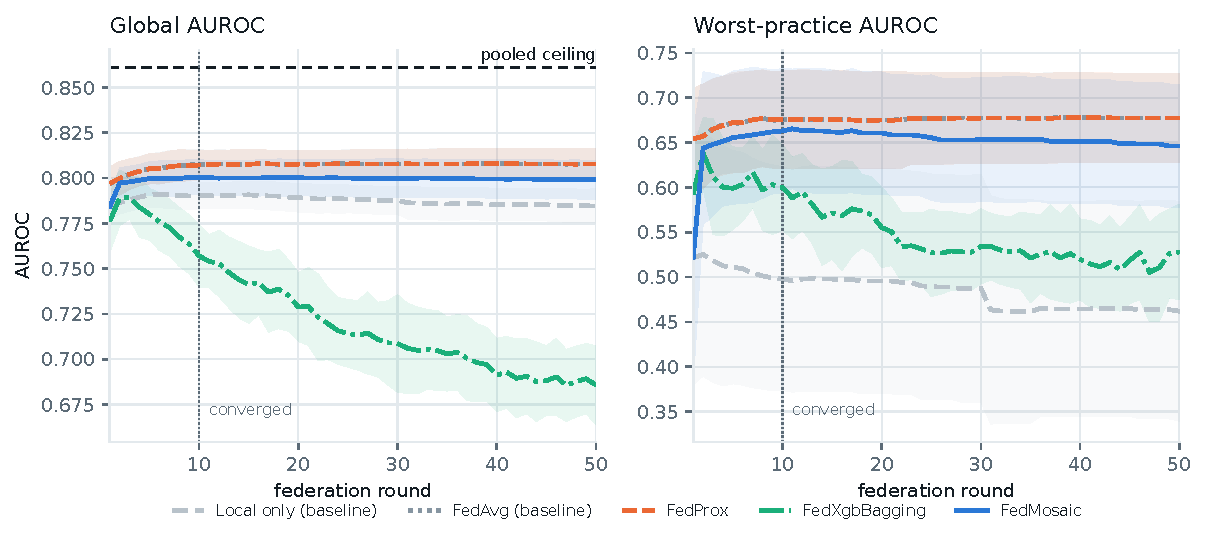
\includegraphics[width=\textwidth]{convergence}
  \caption{AUROC by round, \NumSeeds{} seeds, shaded $\pm$ 1 s.d. The logistic protocols are flat
  from round~10 onward. The tree-based protocol \emph{degrades} with more rounds. FedAvg is not
  missing it lies underneath FedProx, which is the null result reported in
  \S\ref{sec:modelchoice}: the two agree to three decimals.}
  \label{fig:convergence}
\end{figure}

\begin{table}[htbp]
  \centering
  \caption{Accuracy by round count. Nothing after round~10 is bought with the extra privacy loss.}
  \setlength{\tabcolsep}{4.5pt}\small
\begin{tabular}{rrrrrrrrrrr}
    \toprule
    & \multicolumn{5}{c}{Global AUROC} & \multicolumn{5}{c}{Worst practice} \\
    \cmidrule(lr){2-6} \cmidrule(lr){7-11}
    Rounds & Prox & XGB & Mosaic & Local & Avg & Prox & XGB & Mosaic & Local & Avg \\
    \midrule
    5 & 0.805 & 0.780 & 0.800 & 0.791 & 0.805 & 0.672 & 0.599 & 0.655 & 0.511 & 0.671 \\
    10 & 0.807 & 0.757 & 0.800 & 0.790 & 0.807 & 0.675 & 0.600 & 0.663 & 0.498 & 0.676 \\
    20 & 0.808 & 0.729 & 0.800 & 0.789 & 0.808 & 0.675 & 0.555 & 0.661 & 0.495 & 0.675 \\
    35 & 0.808 & 0.703 & 0.800 & 0.786 & 0.808 & 0.677 & 0.521 & 0.653 & 0.462 & 0.677 \\
    50 & 0.808 & 0.686 & 0.799 & 0.785 & 0.808 & 0.677 & 0.528 & 0.646 & 0.462 & 0.677 \\
    \bottomrule
\end{tabular}

  \label{tab:rounds}
\end{table}

Reading the table across rows rather than down columns is the point: for every logistic comparator,
the round-10 figure and the round-\MaxRounds{} figure agree to three decimals. Those forty extra rounds
composed forty extra rounds of privacy loss and returned nothing.

\textbf{The deployment default is now 10 rounds.} At $\sigma = 2.0$ this takes the composed budget
from \EpsAtSigmaTwo{} to approximately 8.1 the largest single improvement available, at zero
accuracy cost and zero engineering risk.

One protocol behaves differently and it is worth noting here because it interacts with the same
lever: the tree-based protocol peaks early and then degrades monotonically, because each round
appends every practice's newly grown trees to one ensemble and, under non-IID data, those trees
encode contradictory local rules. More rounds means more contradiction. For that protocol the round
count is a hyperparameter to tune \emph{down}, not up but \S\ref{sec:modelchoice} recommends
against deploying it at all.

\subsection{The other levers, in order of effect}

\begin{enumerate}
  \item \textbf{Per-practice orchestration of $(b, \sigma)$ landed.} Under any flat DP-SGD
        configuration the composed budget is an accident of practice size: identical settings of
        batch~64 and $\sigma = 1.5$ deliver $\varepsilon = 1.10$ to a 50,000-patient practice and
        $\varepsilon = 16.04$ to a 500-patient one (toy endpoints, ten local epochs; the
        deployment-schedule spread across this report's ten-practice census is 7.25--15.26). The standard's rule-based server planner inverts the shared R\'enyi-DP accountant
        per practice (\S\ref{sec:noise}), so one target $\varepsilon^{*}$ is certified for every
        practice at $\varepsilon^{*} = 2$ the planned $\sigma$ spans 8.32--11.68, and the measured
        utility is flat from $\varepsilon^{*} = 0.5$ to $8$. What used to be ``reduce the budget
        where it hurts'' becomes ``choose the budget once, for everyone''.
  \item \textbf{More practices.} The budget is driven by how much population an individual can hide
        in. Twenty-five practices instead of \NumPractices{} is the pilot's own plan and is the
        structural fix. Under orchestration its effect shows up directly as a smaller required
        $\sigma$ per practice rather than as an easier target.
  \item \textbf{Subsampling amplification.} The standard already credits amplification
        \emph{within} each practice: its Poisson lots sample records at rate $q = b/N_k$, and the
        accountant prices $q$ explicitly. Remaining on the table is amplification \emph{across}
        practices if a practice does not participate in every round, its exposure is further
        amplified away in the accountant's favour. The current configuration has every practice
        train every round, which earns no such credit; the cost of taking it is slower convergence,
        which the round-count finding above suggests there is room to absorb.
  \item \textbf{Accept a larger $\varepsilon$ and let secure aggregation carry the load.} Secure
        aggregation costs bandwidth and coordination, not accuracy (\S\ref{sec:secagg}). At this
        cohort size it protects the individual contribution far more cheaply than noise does, and
        the two are complementary rather than alternatives and they compose in one run:
        \texttt{dpsgd-epsilon} with \texttt{secure-aggregation=true} has been executed live with
        zero failures.
\end{enumerate}

\subsection{What the binding constraint really is}

Throughout, the constraint that binds first is not the mean but the \emph{worst practice}. Global
AUROC degrades gently with noise; the worst practice degrades sharply and with much larger variance.
Since the project's premise is that small practices should get a model they could not build alone,
the worst-practice figure is the one that decides whether a privacy setting is deployable and it
is also the T2.5 fairness measure. Any budget proposal should be evaluated against that column, not
against the headline.

\question{Does the system disclose per-practice information outside the model path?}
\label{sec:sidechannels}
\statusMethod

\begin{shortanswer}
Anonymised logging with a cohort-size floor is the deployment default. No per-practice information
is outside of the model path.
\end{shortanswer}

\paragraph{One residual channel} The export is still ordered by that identifier. The column is
gone, but \emph{row order still follows it}. If identifiers are assigned chronologically, row
position is a weak signal for relative enrolment order. Downstream code does not treat row position
as information. Randomising the order removes the channel at the cost of reproducible extracts; we
have documented the trade-off in the query rather than deciding it unilaterally, because
reproducibility of extractions may matter to the collection protocol.

\question{Does the method work at all what does federation buy, and against what ceiling?}
\label{sec:works}
\statusMeasured

\begin{shortanswer}
Federation reaches \BestFedAUC{} AUROC against a pooled-data ceiling of \CeilingAUC{} a gap of
\CeilingGapAbs{} without any practice sharing a patient row. But the average is not where the
benefit lies. A practice training alone reaches \LocalAUC{} on average while its worst member
manages \LocalWorst{}, which is no better than a coin flip; federation lifts that worst practice to
\BestFedWorst{}, a gain of \WorstGain{}. \textbf{The benefit is equity}, which
matters because the project's premise is that small practices should get a model they could not
build alone.
\end{shortanswer}

\subsection{How the comparison is held fair}

Only the protocol varies. Every comparator sees identical data, identical 80/20 splits, an identical
feature set, an identical local optimiser and identical seeds; each figure is the mean over
\NumSeeds{} seeds. Two reference points make the protocols interpretable, and neither is a protocol:

\begin{itemize}
  \item \textbf{The pooled ceiling} one model trained on every practice's data together. Reality
        forbids it; it is the upper bound federation is trying to reach, and it has no
        worst-practice figure by construction, because pooling destroys the practice boundary the
        measure is defined over.
  \item \textbf{Local-only} each practice trains on its own rows, keeps its own model, and is
        scored on its own held-out rows. This is the honest ``what if we never collaborated'' floor.
\end{itemize}

Two comparisons in the table are deliberately not like-for-like, and reading them as such would
mislead. The tree-based protocol is a different \emph{model class}, reported alongside rather than
head-to-head. And the personalised methods produce \NumPractices{} different models, each scored on
its own practice's patients, whereas the weight-sharing protocols produce a single global model
scored on everyone personalisation is allowed to specialise, so it is measuring something
slightly different.

\begin{table}[htbp]
  \centering
  \caption{Accuracy at \HeadlineRound{} rounds, \NumSeeds{} seeds, mean $\pm$ s.d.
  \NumPractices{} non-IID practices, \NumPatients{} patients.}
  \setlength{\tabcolsep}{5pt}\small
\begin{tabular}{llrrrr}
    \toprule
    & & AUROC & Worst practice & Sensitivity & Uplink bits/round \\
    \midrule
    FedProx & protocol & 0.808 $\pm$ 0.008 & 0.675 $\pm$ 0.054 & 0.703 & 352 \\
    FedAvg (baseline) & baseline & 0.808 $\pm$ 0.008 & 0.675 $\pm$ 0.054 & 0.702 & 352 \\
    FedMosaic & protocol & 0.800 $\pm$ 0.010 & 0.661 $\pm$ 0.068 & 0.709 & 3,600 \\
    Local only (baseline) & baseline & 0.789 $\pm$ 0.008 & 0.495 $\pm$ 0.126 & 0.699 & 0 \\
    \midrule
    \emph{Pooled ceiling} & ceiling & \emph{0.861} & --- & \emph{0.808} & --- \\
    \bottomrule
\end{tabular}

  \label{tab:accuracy}
\end{table}

\begin{figure}[htbp]
  \centering
  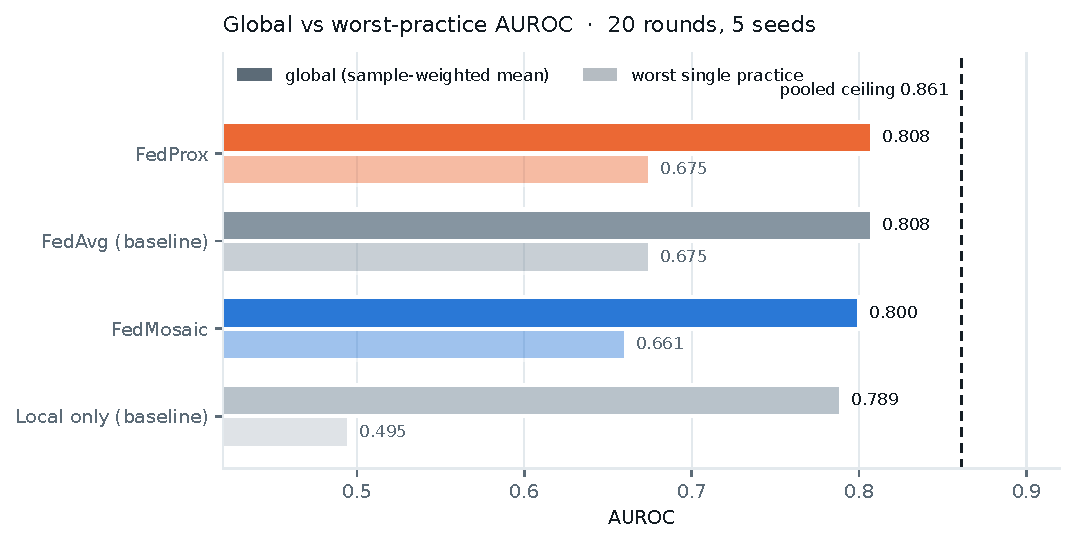
\includegraphics[width=\textwidth]{headline}
  \caption{Global (solid) and worst-practice (pale) AUROC. The gap between the two bars is the
  inequality the project exists to reduce; note how much wider it is for local-only training.}
  \label{fig:headline}
\end{figure}

\subsection{The cohort}

\begin{table}[htbp]
  \centering
  \caption{The synthetic cohort: \NumPractices{} practices, \NumPatients{} patients, panels of
  \PanelMin{}--\PanelMax{}, CKD prevalence \PrevMin{}--\PrevMax{}. This answers the assessment's
  second documented item for the test bed; the pilot's figures will differ (\S\ref{sec:realdata}).}
  \begin{tabular}{rrr}
    \toprule
    Practice & Patients & CKD prevalence \\
    \midrule
    0 & 162 & 10.5\% \\
    1 & 492 & 42.7\% \\
    2 & 434 & 34.6\% \\
    3 & 331 & 42.3\% \\
    4 & 328 & 18.3\% \\
    5 & 532 & 8.3\% \\
    6 & 161 & 46.0\% \\
    7 & 455 & 40.0\% \\
    8 & 216 & 43.5\% \\
    9 & 165 & 21.8\% \\
    \midrule
    Total & 3,276 & \\
    \bottomrule
\end{tabular}

  \label{tab:cohort}
\end{table}

The practices are non-IID in three ways simultaneously covariate shift, label shift and quantity
shift. A \PanelMin{}-patient practice at \PrevMin{} prevalence is a fundamentally different
estimation problem from a \PanelMax{}-patient practice at \PrevMax{}. That is what makes naive
averaging hard, and it is why the worst-practice column moves so much more than the mean.

\subsection{The falsification test}

A result that only ever confirms is not evidence. Every comparator is therefore also run on a
signal-free dataset the same pipeline, the same protocols, but a placeholder table whose maximum
absolute feature--label correlation is \NegControlMaxCorr{}. Anything meaningfully above 0.5 there is a bug, not a
finding.

\begin{table}[htbp]
  \centering
  \caption{Negative control. The highest AUROC any comparator achieves on signal-free data is
  \NegControlMax{}, against a pooled ceiling of \NegControlCeiling{}. Nothing found structure that
  is not there.}
  \begin{tabular}{lrr}
    \toprule
    & AUROC & Worst practice \\
    \midrule
    FedProx & 0.524 $\pm$ 0.030 & 0.260 \\
    FedAvg (baseline) & 0.524 $\pm$ 0.029 & 0.260 \\
    FedMosaic & 0.492 $\pm$ 0.026 & 0.238 \\
    Local only (baseline) & 0.485 $\pm$ 0.041 & 0.266 \\
    \midrule
    \emph{Pooled ceiling} & \emph{0.513} & --- \\
    \bottomrule
\end{tabular}

  \label{tab:negcontrol}
\end{table}

The test passes: no protocol manufactures signal. This is worth recording for counsel because it
bears on whether the headline numbers can be trusted at all the same code, run on data with
nothing in it, reports nothing.

\question{Which model and protocol should the pilot deploy, and why does that matter legally?}
\label{sec:modelchoice}
\statusMeasured

\begin{shortanswer}
Logistic regression under FedProx or FedAvg. The legally useful fact is that this recommendation is
\textbf{over-determined}: the same choice wins on accuracy, on bandwidth, on disclosure surface, and
on protectability. There is no trade-off here in which privacy is bought with performance the
model that federates best is also the only one secure aggregation can protect.
\end{shortanswer}

\subsection{Three findings, one conclusion}

\paragraph{FedProx and FedAvg are indistinguishable.} They agree to three decimals on both measures:
\BestFedAUC{} against \FedAvgAUC{} global, and \BestFedWorst{} worst practice for both. FedProx adds a proximal term
\cite{li2020fedprox} intended to correct client drift, and at two local passes per round there is
almost no drift to correct. This is a null result and is reported as one; it should be retested if
the local epoch count increases, since that is the condition under which the term would start to
matter.

\paragraph{FedMosaic does not win on accuracy, and its case is elsewhere.} It reaches \MosaicAUC{}
global slightly below the weight-sharing protocols, at \UplinkMosaic{} bits per round against
\UplinkLogreg{}. Its argument is its disclosure profile: it
never transmits a model at all, only predictions on an already-public cohort (\S\ref{sec:payload}).
That is a qualitative difference, and if the legal analysis ends up treating parameter vectors as
personal data while treating predictions on public patients differently, FedMosaic becomes worth
revisiting on those grounds not on these.

\paragraph{The tree-based alternative was evaluated and is no longer in scope.} A
gradient-boosted-trees arm (FedXgbBagging) was benchmarked against the logistic protocols on the
pinned run this report is built from: its pooled ceiling matched logistic regression, so the model
class was not the problem, but federated it reached far less, it \emph{degraded} with additional
rounds (\S\ref{sec:reduce}), its split thresholds were literal patient values
(\S\ref{sec:payload}), and secure aggregation could not protect it at all (\S\ref{sec:secagg}).
The measured comparison is retained, marked historical, in the accompanying benchmark report
(the test bed's \texttt{docs/REPORT.md}, scope note 2026-08-28). On 2026-08-28 the tree-based and MLP
code paths were \textbf{deleted from the test bed}; logistic regression --- the model named in
grant task T2.2 --- is now the only model class in the codebase, so the recommendation is not a
preference among alternatives but a description of what exists.

\subsection{Why the convergence matters to counsel}

It is common for privacy measures to be resisted on the grounds that they cost accuracy, which turns
every safeguard into a negotiation. That is not the situation here. The evidence points one way on
every axis at once (numbers as measured on the pinned run; the ``against'' column is the
now-removed trees arm, retained as historical context):

\begin{center}
\small
\begin{tabular}{lll}
  \toprule
  Criterion & Favours & Against (historical) \\
  \midrule
  Global accuracy & logistic regression & trees (removed 2026-08-28) \\
  Worst-practice accuracy & logistic regression & trees (removed 2026-08-28) \\
  Behaviour with more rounds & logistic regression (flat) & trees (degrade) \\
  Bandwidth & logistic regression & trees ($\sim$60$\times$ the uplink) \\
  Disclosure surface & logistic regression & trees (literal patient values) \\
  Protectable by secure aggregation & logistic regression & trees (impossible) \\
  \bottomrule
\end{tabular}
\end{center}

The consortium therefore does not have to trade model performance for the ability to make privacy
guarantees. Pinning the deployment to logistic regression is what makes secure aggregation possible
at all, and it costs nothing to do so.

\input{sections/12-anonymisation-test}
\question{What changes when real practice data replaces the synthetic cohort?}
\label{sec:realdata}
\statusMeasured

\begin{shortanswer}
Structurally, nothing: who sees what, what is on the wire, and whether secure aggregation and DP
apply are properties of the protocol, not of the data. Every accuracy number is expected to move
up, and the leakage audit must be re-run, and only the twenty-five-practice cohort will tell us
whether a meaningful privacy budget is reachable at all.
\end{shortanswer}

\subsection{What are we predicting?}

The synthetic label is \textbf{CKD stage $\ge$ 3 prevalence} does this patient have it now. The
production contract defines \textbf{incidence}: among patients with no prior CKD diagnosis at a
rolling landmark date, does one appear within the following year.

\subsection{Which conclusions survive the move, and which do not}

\begin{center}
\small
\begin{tabular}{p{6.6cm}p{6.6cm}}
  \toprule
  \textbf{Data-invariant holds for the pilot} & \textbf{Data-dependent must be re-measured} \\
  \midrule
  The aggregating party receives individual, attributable updates unless secure aggregation is
  enabled (\S\ref{sec:isolation})
  & Every AUROC figure, global and worst-practice \\
  \addlinespace
  Central DP does not change what the server receives; only local DP does (\S\ref{sec:noise})
  & The achievable $\varepsilon$, which depends on real cohort sizes \\
  \addlinespace
  Payload shape per protocol, and that tree split thresholds are literal patient values
  (\S\ref{sec:payload})
  & The utility cost of local DP at the pilot's scale \\
  \addlinespace
  Secure aggregation is available, semi-honest, leaves participation visible, and cannot protect
  trees (\S\ref{sec:secagg})
  & The membership-inference result, with eGFR present (\S\ref{sec:anontest}) \\
  \addlinespace
  Flower Labs has no access path in a self-hosted deployment (\S\ref{sec:flowerlabs})
  & Whether logistic regression remains the right model class \\
  \addlinespace
  Fewer rounds reduces the budget proportionally
  & How many rounds convergence actually needs on real data \\
  \bottomrule
\end{tabular}
\end{center}

\question{What lies outside this report's technical scope?}
\label{sec:outside}
\statusOutside

\begin{shortanswer}
There are four questions that need to be answered
\end{shortanswer}

\subsection{A decision the consortium has not yet taken}

The allocation of controller, joint-controller and processor roles under Art.~26/28 turns on
\textbf{who operates the SuperLink host} is docport, or IKIM/KITE. That decision has not been made,
so the question is not merely legal but not yet decidable. The technical facts bearing on it:

\begin{itemize}
  \item Whoever operates the host is the party that, on the default configuration, receives
        individual attributable updates (\S\ref{sec:isolation}).
  \item With secure aggregation enabled, that party receives only the aggregate which may
        materially change the analysis, and is the strongest reason to take the configuration
        decision early rather than at Milestone~4.
  \item The node registry mapping public keys to admitted practices is centrally held by that
        operator, independently of the model path.
\end{itemize}

\subsection{Facts about a deployment that does not exist}

The assessment's fourth documented item administrative access, logging and export capabilities
on the SuperLink is the one item this report cannot close. We can document the full
\textbf{capability surface}, and Appendix~\ref{sec:config} does: the state database, log files and
rotation, run log retrieval, run listing and termination, and the node registry commands.

Also, the \textbf{real per-practice cohort sizes}, which are an MS3/MS5 fact about the world
and the input that decides whether a meaningful budget is reachable; and the \textbf{practices' own
IT environments}.

\section{Recommendations}
\label{sec:recs}

Ordered by effect on the legal position per unit of engineering effort. Items 1--5 are done and are
listed so that the record is complete; 6--12 are open.

\subsection*{Completed since the assessment}

\begin{enumerate}
  \item \textbf{Implement secure aggregation} and verify it end-to-end. Converts the answer to the
        central question from ``the server sees individual updates'' into a configuration choice.
        (\S\ref{sec:secagg})
  \item \textbf{Implement and measure local DP.} Establishes what noise-at-the-practice actually
        costs rather than asserting availability. The update-level answer is uncomfortable and is
        reported as such; item~5 is its resolution. (\S\ref{sec:noise})
  \item \textbf{Build the membership-inference audit}, with a positive control. Converts ``DP is
        configured'' into a reported attack result. (\S\ref{sec:anontest})
  \item \textbf{Close the two side channels} the direct identifier in the export, and identified
        per-practice metric logging, now anonymised by default. (\S\ref{sec:sidechannels})
  \item \textbf{Ship the deployment standard: logistic regression with record-level DP-SGD inside
        each practice, SecAgg+ on the wire, and per-practice $\varepsilon$ orchestration by a
        rule-based server agent.} The planner is deterministic — a rule table, not a model; no LLM
        is involved anywhere in the stack. R1~\emph{inventory}: read each practice's census $N$,
        the only datum exchanged; R2~\emph{fixed global policy}: one target
        $(\varepsilon^{*},\, \delta = 10^{-5})$ for the whole federation; R3~\emph{per-practice
        inversion}: for each practice, invert the shared R\'enyi-DP accountant for the batch size
        and smallest $\sigma$ that certify $\varepsilon \le \varepsilon^{*}$; R4~\emph{dispatch}:
        issue each practice's plan as ordinary run configuration. Measured utility is flat from
        $\varepsilon^{*} = 0.5$ to $8$ (\S\ref{sec:noise}), and the standard composes with secure
        aggregation in one live run, zero failures (\S\ref{sec:secagg}). This closes the
        engineering question of whether a meaningful in-practice privacy guarantee is reachable;
        the choice of $\varepsilon^{*}$ itself remains a policy decision for the consortium, which
        this report deliberately does not make. (\S\ref{sec:noise}, \S\ref{sec:reduce})
\end{enumerate}

\subsection*{Open, in priority order}

\begin{enumerate}[start=6]
  \item \textbf{Decide who operates the SuperLink, and decide secure aggregation with it.} These are
        the same decision viewed from two sides, they gate the Art.~26/28 analysis, and they have the
        longest lead time of anything on this list. (\S\ref{sec:outside})
  \item \textbf{Build the remaining two attack families} model inversion and reconstruction
        so that the audit covers what EDPB Opinion 28/2024 actually names. Consider also a
        likelihood-ratio attack as a stronger membership test. (\S\ref{sec:anontest})
  \item \textbf{Obtain the analytics work package's indicator specification} and apply the same
        accountant and a cell-suppression analysis to it. Until then, half of the assessment's
        framing is unanswered.
  \item \textbf{Confirm the round count on real data.} Convergence by round~10 is the cheapest
        privacy improvement available and it is currently a synthetic-data finding.
        (\S\ref{sec:reduce})
  \item \textbf{Evaluate practice-level subsampling amplification.} The standard already credits
        record-level Poisson subsampling within each practice; participation below 1.0 across
        rounds would earn a further budget reduction the accountant can credit. The cost is
        convergence speed. (\S\ref{sec:reduce})
  \item \textbf{Re-run the whole evidence base on the pilot cohort} once real data exists
        accuracy, budget and audit alike. The right-hand column of \S\ref{sec:realdata} is the
        checklist.
  \item \textbf{Implement FedMosaic's own DP construction} if that protocol is to be considered on
        privacy grounds, since its current case rests on payload shape alone. (\S\ref{sec:payload})
\end{enumerate}

\subsection*{Mapping to the project plan}

\begin{center}
\small
\begin{tabular}{lll}
  \toprule
  Item & Work package & Milestone \\
  \midrule
  Secure aggregation (1), operator decision (6) & T2.3 & MS4 (month 18) \\
  DP measurement (2), deployment standard (5), amplification (10) & T2.3 & MS4 \\
  Leakage audit (3), remaining attacks (7) & T2.5 & MS4 onward \\
  Side channels (4) & T2.3 / data collection & before MS3 \\
  Analytics indicator spec (8) & analytics work package &  \\
  Re-run on pilot cohort (11) & T2.4 & MS5 (month 24) \\
  \bottomrule
\end{tabular}
\end{center}

\appendix

\section{Reproducibility}
\label{sec:repro}

Every figure, table and inline number in this report is produced by one script from one run. No
quantity is typed into the prose by hand: each resolves through a generated macro, so the document
cannot drift from the data it describes.

\begin{center}
% GENERATED by paper/make_paper.py -- do not edit.
\begin{tabular}{ll}
    \toprule
    Item & Value \\
    \midrule
    Run date & 2026-08-20 \\
    Python & 3.11.11 \\
    \texttt{flwr} & 1.33.0 \\
    \texttt{numpy} & 2.4.6 \\
    \texttt{scikit-learn} & 1.8.0 \\
    Seeds & 42, 43, 44, 45, 46 \\
    Rounds recorded & 50 (headline read at 20) \\
    DP / audit rounds & 20 \\
    \bottomrule
\end{tabular}

\end{center}

\subsection{Reproducing this report}

\begin{verbatim}
uv sync --extra dev --extra notebook
uv run ckd-clinics --clinics 10
uv run python paper/make_paper.py --recompute
\end{verbatim}

\subsection{A reproducibility defect in the earlier figures, and its correction}

\textbf{Any privacy figure quoted from project documentation dated before this report should be
re-checked.} The earlier DP tables could not be reproduced from their stated seeds, and three
documents in the repository disagreed about them.

The cause was a single unseeded step. Flower draws its differential-privacy noise from NumPy's
\emph{global} legacy random generator. This project's seed reached the train/test split but never
that generator, so the DP noise was the one unseeded step in an otherwise fully seeded pipeline. The
signature was unmistakable in hindsight: the zero-noise row draws no noise and was bit-identical
across all three documents, while disagreement grew with the noise level.

The generator is now seeded per (seed, noise level) cell before each run per cell rather than
once per run, because the noise stream is consumed sequentially, so a single per-run seed would make
every row depend on which noise levels precede it in the sweep. Each of the \NumSeeds{} seeds still
draws different noise, so the error bars retain their meaning.

\textbf{Verification.} Running the pipeline twice in independent processes now reproduces every
number bit-identically. This check is the first gate in the build and it failed, by construction,
before the correction.

\section{Configuration reference}
\label{sec:config}

\subsection{Training and aggregation}

This is the assessment's third documented item, in full. It is a single declarative block, versioned
with the code it configures, so any run's configuration is recoverable from the commit that produced
it.

\begin{center}
\small
\setlength{\tabcolsep}{4pt}
\begin{tabular}{llp{7.4cm}}
  \toprule
  Key & Value & What it does \\
  \midrule
  \texttt{num-server-rounds} & 10 & Federation rounds. Reduced from 20 see \S\ref{sec:reduce} \\
  \texttt{num-practices} & 12 & Simulated SuperNodes (must equal \texttt{options.num-supernodes}) \\
  \texttt{alpha} & 0.5 & Dirichlet non-IID concentration for the synthetic split \\
  \texttt{iid} & false & Even-split ablation switch \\
  \texttt{fraction-fit} & 1.0 & Fraction of practices training per round \\
  \texttt{local-epochs} & 2 & Local passes per round \\
  \texttt{model} & \texttt{logreg} & Logistic regression (\S\ref{sec:modelchoice}) \\
  \texttt{class-weight-balanced} & true & Corrects the prevalence imbalance \\
  \texttt{seed} & 42 & One global seed; per-practice seeds derived from it \\
  \texttt{data-source} & \texttt{csv} / \texttt{fhir} & Where each practice reads its own rows \\
  \midrule
  \texttt{metric-privacy} & \textbf{true} & Anonymise per-practice metric lines (\S\ref{sec:sidechannels}) \\
  \texttt{min-cohort-size} & \textbf{20} & Suppress lines below this cohort floor \\
  \texttt{min-train-examples} & 0 & Participation floor (0 = off in the research baseline) \\
  \texttt{central-dp-epsilon} & 0.0 & Server-side noise at aggregation; 0 = off (\S\ref{sec:budget}) \\
  \texttt{central-dp-delta} & 1e-5 & $\delta$ for the central-DP accountant inversion \\
  \texttt{local-dp-epsilon} & 0.0 & Update-level noise inside the SuperNode; 0 = off (\S\ref{sec:noise}) \\
  \texttt{dpsgd-epsilon} & 0.0 & Record-level DP-SGD target $\varepsilon^{*}$; 0 = off. Activates the
        orchestrated standard: the server planner issues per-practice \texttt{batch-size} and
        \texttt{noise-multiplier} from the census (\S\ref{sec:noise}, \S\ref{sec:reduce}) \\
  \texttt{secure-aggregation} & false & SecAgg+ masking (\S\ref{sec:secagg}) \\
  \texttt{secagg-num-shares} & 3 & Shamir shares issued per practice \\
  \texttt{secagg-reconstruction-threshold} & 2 & Shares needed to recover a dropped mask \\
  \bottomrule
\end{tabular}
\end{center}

Differential privacy parameters not in the run config: clipping norm $C = 1.0$, $\delta = 10^{-5}$
(chosen below $1/n$), accountant R\'enyi-DP via \texttt{dp\_accounting} \cite{dpaccounting}. The
DP-key relations enforced in \texttt{server\_app.main}: \texttt{dpsgd-epsilon} rejects
both \texttt{central-dp-epsilon} and \texttt{local-dp-epsilon} (the record-level budget would be
spent twice), and \texttt{central-dp-epsilon} rejects \texttt{secure-aggregation} (masking arrives
before central DP's server-side noising reads the updates). The remaining pair
(\texttt{central-dp-epsilon} + \texttt{local-dp-epsilon}) is allowed: stacked noise only
over-protects at a utility cost, never over-spends budget. \texttt{dpsgd-epsilon} \emph{with}
\texttt{secure-aggregation} is the standard's own combination and is verified live.

\subsection{SuperLink capability surface}

The assessment's fourth documented item, to the extent it is answerable without a deployment
(\S\ref{sec:outside}). These are capabilities of the software an operator would inherit, not
observations of a running host no such host exists.

\begin{center}
\small
\begin{tabular}{lp{7.2cm}}
  \toprule
  Surface & What an operator would have \\
  \midrule
  State database & Run state persisted to a file on the host; omitting the option keeps state in
                   memory only, lost on restart \\
  Log file and rotation & Server logs written to disk, with rotation interval and backup count \\
  Run log retrieval & Any operator with control-API access can pull a run's logs \\
  Run listing and termination & Enumerate and stop runs \\
  Node registry & The mapping of public keys to admitted practices is centrally held and
                  administrable \\
  \bottomrule
\end{tabular}
\end{center}

\section{Limitations}
\label{sec:limits}

\begin{center}
\small
\begin{tabular}{p{6.2cm}p{7.0cm}}
  \toprule
  Limitation & Consequence \\
  \midrule
  Synthetic data throughout & No absolute figure here is a clinical claim \\
  No eGFR & The strongest CKD predictor is missing; real data should lift every accuracy number and
            may weaken the leakage result \\
  Prevalence, not incidence & A different prediction task from the production contract
            (\S\ref{sec:realdata}) \\
  \NumPractices{} practices, not 25 & Understates the pilot, especially for the privacy budget \\
  Leakage audit covers 1 of 3 attack families & Not a demonstration of anonymity
            (\S\ref{sec:anontest}) \\
  Fairness audited by age band, not sex & The specified analysis is impossible until real data
            arrives \\
  DP measured on federated averaging only & FedProx and FedMosaic DP costs unmeasured \\
  Secure aggregation verified in simulation & Not yet exercised against a live multi-host SuperLink \\
  \bottomrule
\end{tabular}
\end{center}


\printbibliography[heading=bibintoc]

\end{document}
